\chapter{Estado del arte} \label{sec:cap2}

\noindent El estudio del movimiento del cuerpo humano es una tarea compleja, que requiere de amplios conocimientos en el sector de la biomecánica, y herramientas específicas para su análisis. En este sentido, el sistema de captura de movimiento, conocido como \textit{Motion Capture} (MoCap), es una herramienta fundamental para el estudio del movimiento humano \autocite{taiQueEsMotion2024}.


\section{Sistemas \textit{Motion Capture}}
\noindent El \textit{Motion Capture} es una técnica que permite capturar el movimiento de un objeto en tiempo real, y representarlo en un entorno virtual. Esta técnica se utiliza en diferentes campos, como la animación, la medicina, la biomecánica o la robótica; y se basa en la captura de la posición de diferentes marcadores en el espacio. Para lograr la captura, existen diferentes tecnologías, como cámaras de vídeo, sensores inerciales, sensores de ultrasonidos, etc. \autocite{taiQueEsMotion2024}

\subsection{\textit{Hardware} disponible}
\noindent En la facultad de INEF de la UPM, se utiliza un sistema de Motion Capture basado en cámaras de infrarrojo, que utilizan para capturar movimientos deportivos\footnote{La facultad de INEF cuenta con 6 cámaras infrarrojas de la marca Vicon, capaces de capturar fotogramas a una frecuencia de hasta 500 Hz \autocite{FacultadCienciasActividad}}. Estos marcadores se colocan en diferentes partes del cuerpo del deportista, logrando capturar un movimiento preciso. Los datos capturados se almacenan en un fichero en formato C3D, que contiene la información necesaria para la representación del movimiento. \todo{Añadir mas info sobre el sistema Vicon de INEF}

Las tecnologías que existen en el mercado para la visualización de estos movimientos son muy costosas, y no siempre se adaptan a las necesidades de los investigadores. Por ello, en este proyecto se ha desarrollado una aplicación para la visualización de movimientos capturados en formato C3D. La aplicación permite la visualización de los movimientos en un entorno tridimensional, pudiendo variar diferentes parámetros de la visualización, como la velocidad de reproducción, la posición de la cámara, la representación de los marcadores, de las uniones, vectores o fuerzas.

Es relevante señalar que este Proyecto se ciñe al sistema MoCap disponible en la facultad de INEF de la UPM, por el elevado coste de estos sistemas y la imposibilidad de trabajar con alternativas de la competencia. Sin embargo, existen otras alternativas con gran aceptación en el mercado.

\subsection{Alternativas}
\noindent Existen diferentes alternativas a los sistemas Vicon disponibles en el mercado, como los sistemas OptiTrack o Qualisys. En el artículo \autocite{article} se comparan estos sistemas, quedando patente que estos sistemas son capaces de capturar correctamente el movimiento. Además, en la \autoref{fig:errores-mocap} se aprecia como los errores de estos sistemas se han ido reduciendo a lo largo del tiempo.

\begin{figure}[H]
    \centering
    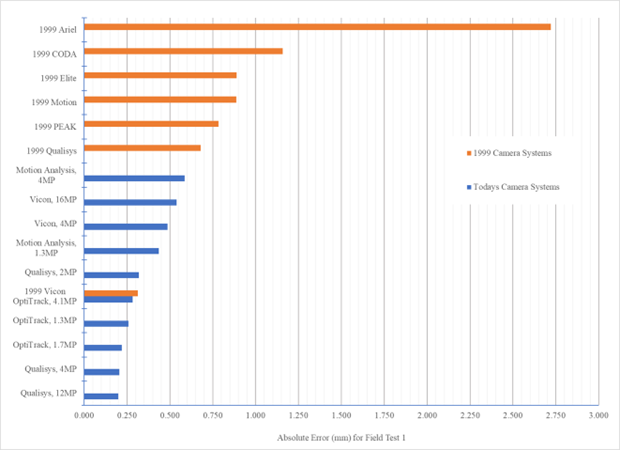
\includegraphics[width=\textwidth]{errores-mocap.png}
    \caption{Error absoluto de diferentes sistemas. Obtenido de \autocite{article}.}
    \label{fig:errores-mocap}
\end{figure}

\section{Ficheros C3D} \label{sec:ficheros-c3d}

\noindent Entender el formato de los ficheros C3D es fundamental para el desarrollo de esta aplicación. 

El formato C3D es un formato de fichero binario de dominio público que se crea a mediados de los años 80, en el \textit{National Institutes of Health Biomechanics Laboratory}, en Maryland, USA, y es compatible con todos los principales sistemas de captura de movimiento 3D. Es usado por empresas de las industrias de biomecánica, captura de movimiento y animación \autocite{C3DORGBiomechanicsStandard}.

Un fichero C3D es un fichero binario que contiene toda la información de la captura de movimiento. Como se explica en \autocite{C3DORGBiomechanicsStandard}, este fichero se compone de diferentes secciones, que contienen la información de los marcadores para cada fotograma de la captura. Existen diferentes \textit{parsers} que permiten la lectura de estos ficheros, y la extracción de la información necesaria para la representación del movimiento. En este proyecto se ha utilizado el \textit{crate} \texttt{c3dio}, que permite la lectura de ficheros C3D en Rust, y tiene un \textit{plugin} para \texttt{Bevy} que facilita la integración con el motor de videojuegos, que se explica en el \autoref{subsec:bevy}.

\subsection{Herramientas actuales para la visualización de ficheros C3D}

\noindent Las herramientas actuales que existen en el mercado para la visualización de un fichero C3D son escasas y generalmente costosas. Una biblioteca famosa en el pasado para el tratamiento de ficheros C3D era la \textit{Biomechanics ToolKit} - BTK, pero fue comprada por la compañía canadiense \textit{Movec}, que tiene intención de renovarla bajo el nombre comercial \textit{Bridge} \autocite{Bridge,ProjectBiomechanicalToolKit}.

\section{Lenguaje de programación}

\noindent Como se explica en el \autoref{sec:ficheros-c3d}, un fichero C3D contiene toda la información de la posición de los marcadores a lo largo de la grabación del movimiento. Una frecuencia de muestreo típica en este tipo de ficheros es de 250 Hz, lo que significa que se captura la posición de los marcadores 250 veces por segundo. Adicionalmente, al fichero C3D se le añaden puntos calculados, que pueden ser articulaciones entre dos marcadores reales, vectores de velocidad, aceleraciones, etc. Por tanto, es común que un fichero C3D contenga miles de puntos, lo que hace que la visualización de estos movimientos sea una tarea compleja y exigente en términos de rendimiento.  

Adicionalmente, en el planteamiento del proyecto, se especificó que debían existir dos versiones, una de escritorio y una versión web. Con estas premisas, se han valorado diferentes lenguajes de programación para el desarrollo de la aplicación.  

\subsection{JavaScript}
\noindent JavaScript es un lenguaje de programación interpretado, que se ha convertido en el estándar para el desarrollo de aplicaciones web. Este lenguaje es eficiente y rápido, gracias a optimizaciones en los motores de JavaScript, como SpiderMonkey de Mozilla o V8 de Google \autocite{srinetChromeV8Firefox2022}. Para el desarrollo de aplicaciones de escritorio, JavaScript se puede utilizar con diferentes tecnologías, como Electron \autocite{BuildCrossplatformDesktop}, que permite la creación de aplicaciones de escritorio multiplataforma con tecnologías web. Pese a esto, el mayor problema de JavaScript es el rendimiento, ya que este lenguaje no dispone de características de bajo nivel, como la gestión de memoria o la programación concurrente \autocite{MemoryManagementJavaScript2025,pengMultithreadingJavascript2017}.

\subsection{Python}
\noindent Python es un lenguaje de programación interpretado, que se ha convertido en uno de los lenguajes de programación más populares en la actualidad \autocite{TIOBEIndex}. Python es un lenguaje de programación de tipado dinámico, que permite la inferencia de tipos, y que garantiza la seguridad de la memoria en tiempo de ejecución. Python es un lenguaje de programación muy versátil, que se utiliza en diferentes campos, como la inteligencia artificial, el análisis de datos, la programación web, etc. Además, dispone de una gran cantidad de bibliotecas y frameworks, que facilitan el desarrollo de aplicaciones de todo tipo. Sin embargo, Python no es un lenguaje de programación especialmente rápido, ya que es un lenguaje interpretado, y generalmente sus bibliotecas son pesadas y poco eficientes, por lo que se suele considerar un lenguaje ideal únicamente para prototipado \autocite{SlowestProgrammingLanguages2020}.

\subsection{C++}
\noindent C++ es un lenguaje de programación de propósito general, que se utiliza en diferentes campos, como la programación de sistemas, la programación de videojuegos, la programación de aplicaciones de escritorio, etc. C++ es un lenguaje de programación de tipado estático, que permite la inferencia de tipos, y que garantiza la seguridad de la memoria en tiempo de compilación. C++ es un lenguaje de programación muy eficiente, que permite la programación de bajo nivel, y que dispone de una gran cantidad de bibliotecas y frameworks, que facilitan el desarrollo de aplicaciones de todo tipo. C++ es un lenguaje de programación muy rápido, que se utiliza en aplicaciones que requieren un alto rendimiento, como videojuegos, motores de renderizado, sistemas operativos, etc. Sin embargo, C++ es un lenguaje de programación antiguo, que no dispone de características modernas, como un gestor de paquetes para la gestión de dependencias. Además, C++ no es un lenguaje de programación concebido para el desarrollo de aplicaciones web.

\subsection{Rust}
\noindent El lenguaje de programación Rust es un lenguaje de programación innovador que prioriza la seguridad y la eficiencia. Este lenguaje ha sido diseñado por Mozilla Research, y se ha convertido en uno de los lenguajes de programación más populares en la actualidad. Rust es un lenguaje de programación multiparadigma, que combina elementos de programación funcional, orientada a objetos e imperativa. Rust es un lenguaje de programación de tipado estático, que permite la inferencia de tipos, y que garantiza la seguridad de la memoria en tiempo de compilación. 

Rust dispone de características modernas, como un gestor de paquetes para la gestión de dependencias, llamado Cargo, y compilación nativa a WebAssembly, lo que permite la ejecución de código Rust en un navegador web \autocite{WebAssembly}.

\subsection{Otras herramientas consideradas}
\subsubsection{Unity}
\noindent Unity es un motor de videojuegos multiplataforma, que permite el desarrollo de videojuegos en 2D y 3D. Unity es un motor de videojuegos muy popular, que se puede utilizar también como herramienta crear simulaciones, que es el propósito de este proyecto. Unity dispone de una gran cantidad de herramientas y bibliotecas, que facilitan el desarrollo de aplicaciones de todo tipo. Sin embargo, Unity es un motor de videojuegos pesado, que consume muchos recursos, y que no es especialmente eficiente en términos de rendimiento, sobre todo en entornos web.

\section{Comparativa de rendimiento}

\begin{figure}[H]
    \centering
    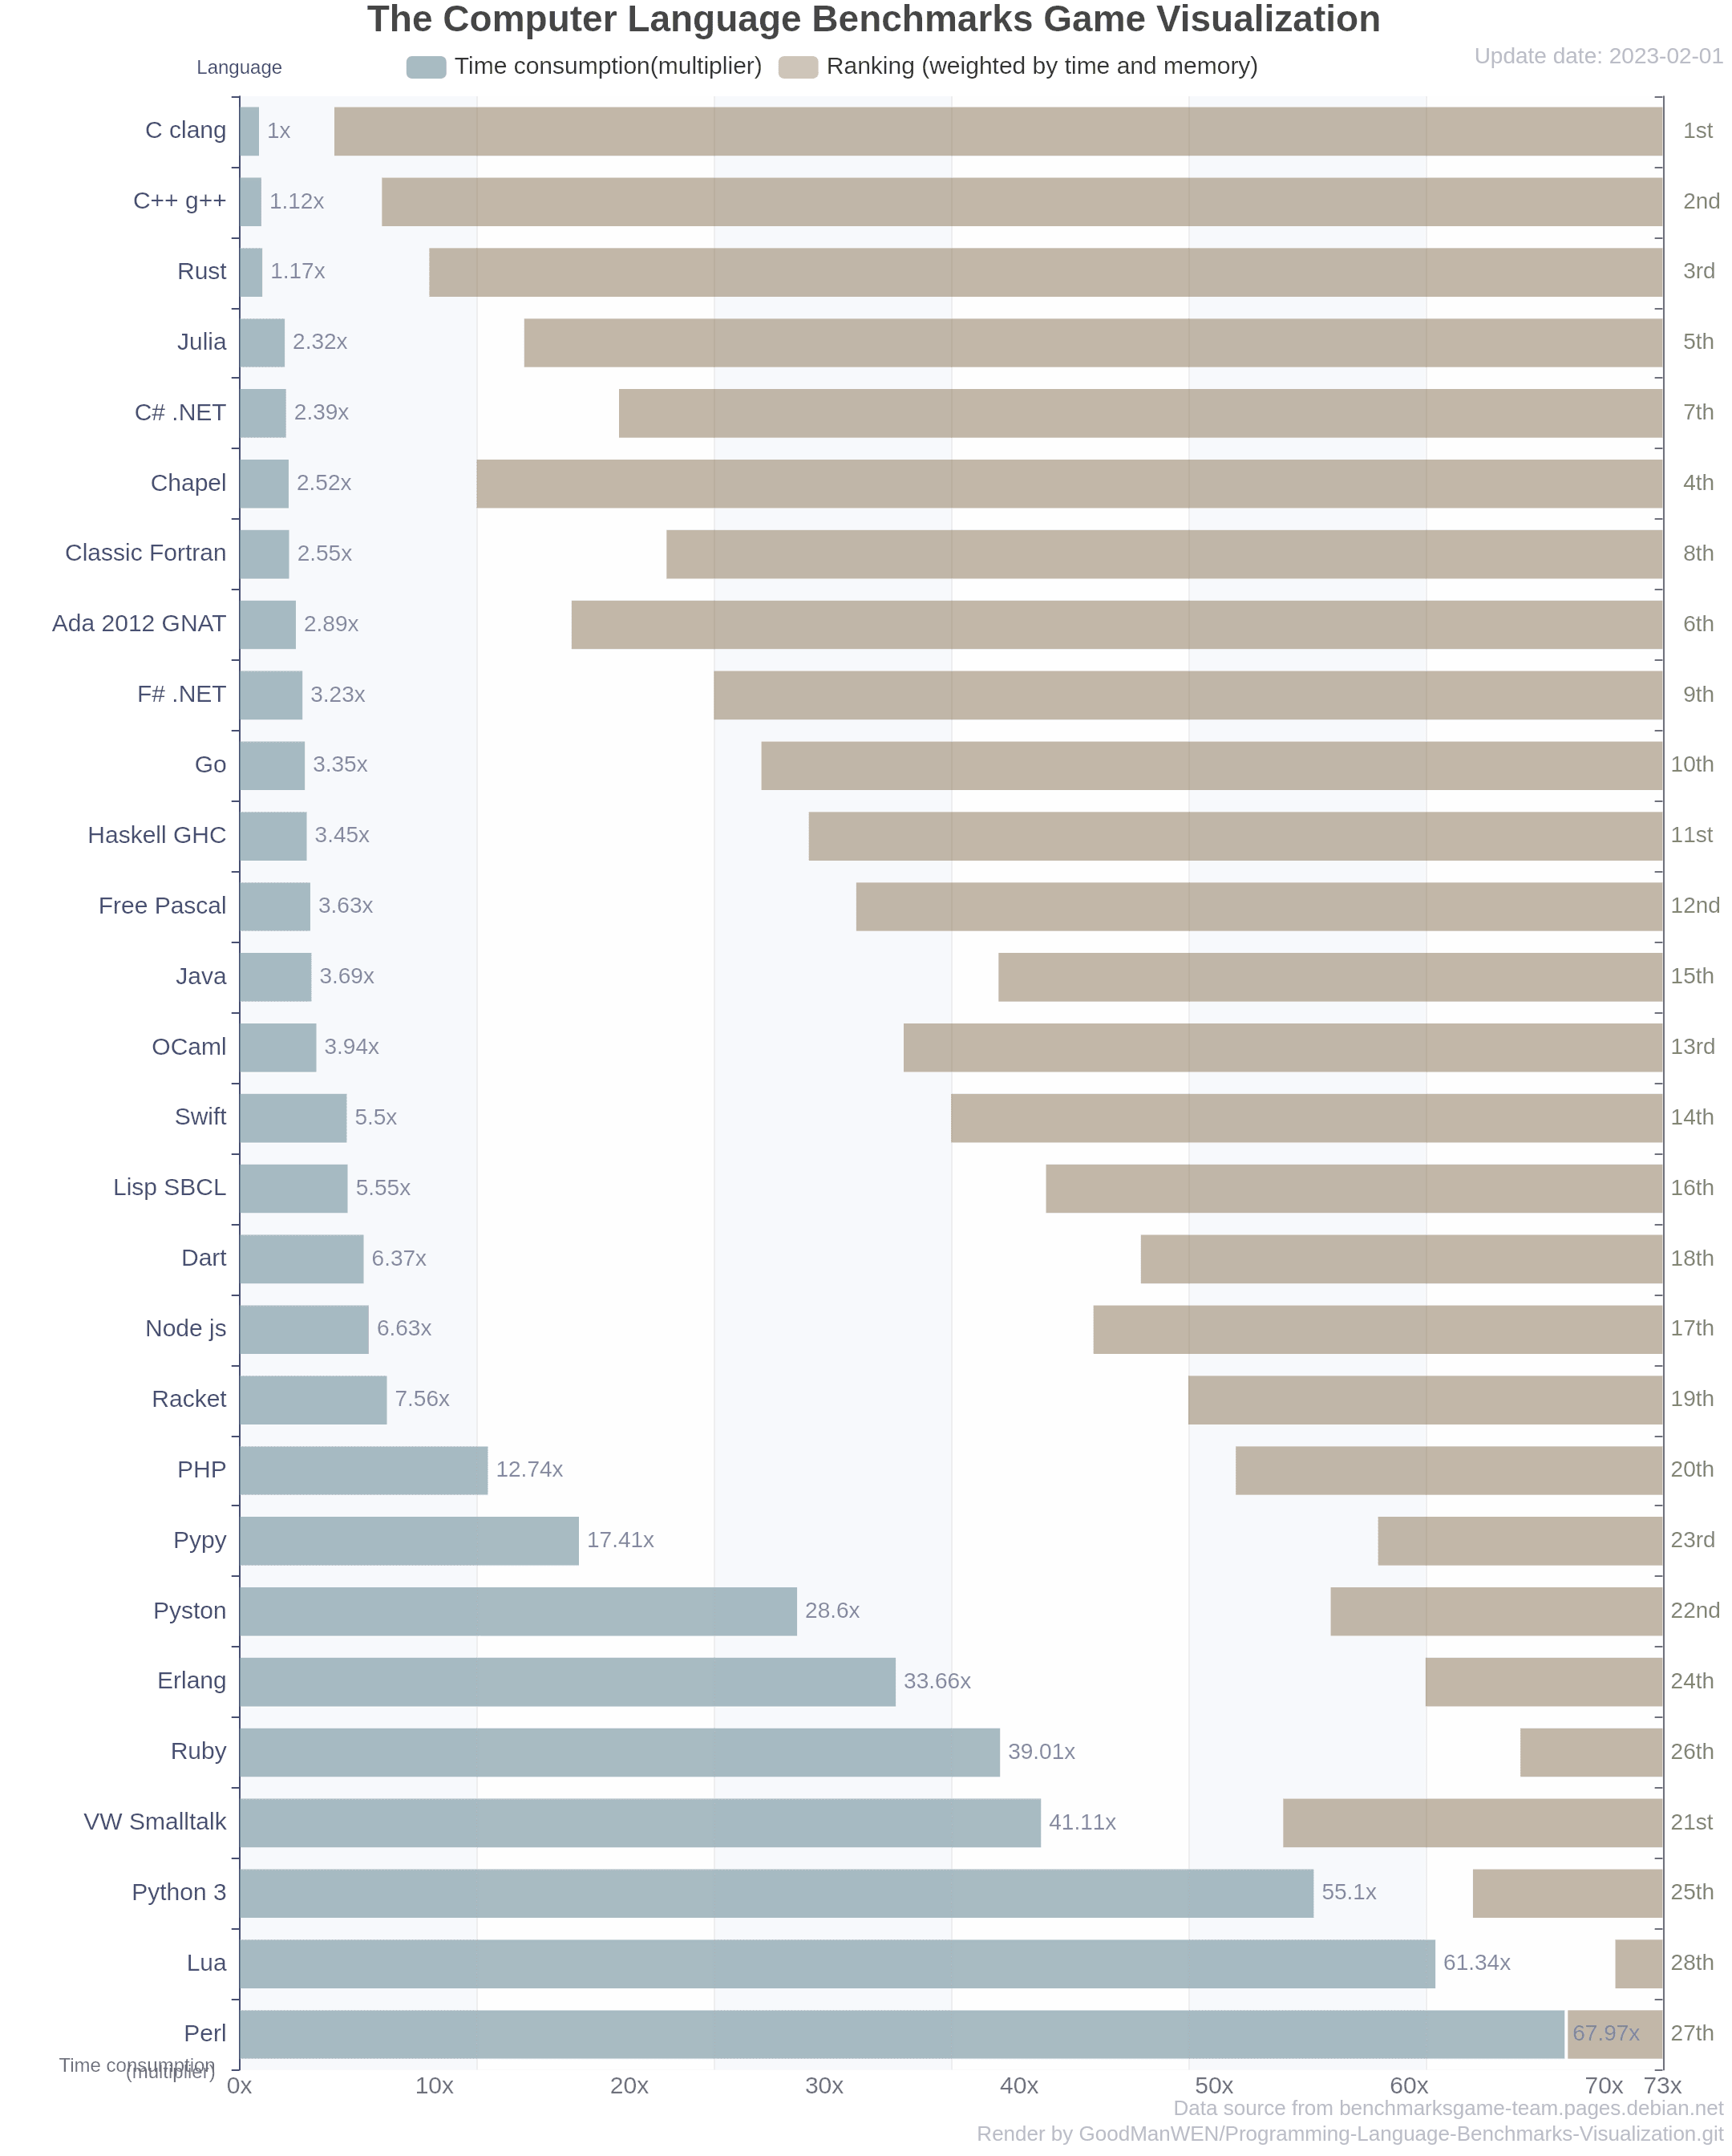
\includegraphics[width=\textwidth]{comparativa rendimiento lenguajes.png}
    \caption{Comparativa de rendimiento en entornos de escritorio \autocite{zotero-16}}
    \label{fig:comparativa-rendimiento}
\end{figure}

% https://goodmanwen.github.io/Programming-Language-Benchmarks-Visualization/

\noindent Como se puede observar en la \autoref{fig:comparativa-rendimiento}, que coincide con el análisis de \autocite{samTop10Fastest2024}, Rust cae en los primeros puestos por rendimiento, teniendo un rendimiento similar al de C y C++, y superando ampliamente a Python y Node.js (\textit{JavaScript}).

Sin embargo, esta tabla no es válida en entornos web, dado que en estos entornos el rendimiento de los diferentes lenguajes de programación se ve limitado por características propias de los navegadores. Por ejemplo, Rust compilado a WebAssembly no tiene acceso directo al DOM (\textit{Document Object Model}, el modelo de objetos de un documento HTML). Esto significa que Rust no puede manipular directamente los elementos de la página web, y que necesita comunicarse con JavaScript para hacerlo. 

Un \textit{benchmark} de rendimiento en entornos web se puede encontrar en \autocite{InteractiveResults}, que muestra que \textit{vanilla JavaScript} es el lenguaje más rápido en este tipo de entornos. Sin embargo, en un proyecto como este, no se contempla el uso de \textit{vanilla JavaScript}, puesto que se necesita un \textit{framework} que permita la creación de aplicaciones gráficas de forma sencilla y eficiente. Si se analiza el rendimiento de diferentes \textit{frameworks} en entornos web, se puede ver que la diferencia entre los basados en \textit{JavaScript} y los basados en \textit{Rust} es mínima, no habiendo un claro vencedor en este aspecto \autocite{InteractiveResults}.

\section{Elección del lenguaje de programación}

\noindent Valorando las diferentes opciones, se ha decidido utilizar Rust para el desarrollo de la aplicación. Las características que han sido determinantes en la elección de Rust son las siguientes:

\begin{enumerate}
    \item \textbf{Seguridad:} Rust es un lenguaje de programación que garantiza la seguridad de la memoria en tiempo de compilación, lo que evita errores comunes en la programación, como los desbordamientos de búfer o las fugas de memoria.
    \item \textbf{Eficiencia:} Rust es un lenguaje de programación muy eficiente, que permite la programación de bajo nivel, y que garantiza un alto rendimiento en la ejecución del código.
    \item \textbf{Modernidad:} Rust es un lenguaje de programación moderno, que dispone de características avanzadas, como un gestor de paquetes para la gestión de dependencias, y compilación nativa a WebAssembly.
    \item \textbf{Versatilidad:} Rust es un lenguaje de programación multiparadigma, que combina elementos de programación funcional, orientada a objetos e imperativa, lo que facilita el desarrollo de aplicaciones de todo tipo.
\end{enumerate}

\section{Herramientas de desarrollo}
\noindent Para conseguir una aplicación gráfica eficiente, se debe de contar con una interfaz que permita a la aplicación trabajar con el hardware del dispositivo. Por tanto, es importante utilizar herramientas multiplataforma que permitan a la aplicación ser eficiente en diferentes entornos. En Rust, existen muchos \textit{crates} (unidades de compilación, ver \autocite{PackagesCratesRust}) que permiten el desarrollo de aplicaciones gráficas, como \texttt{wgpu} \autocite{WgpuPortableGraphics}, \texttt{glium} \autocite{GliumGlium2025}, \texttt{piston} \autocite{PistonModularOpen}, etc. Sin embargo, estos \textit{crates} son de muy bajo nivel, y crear una aplicación gráfica desde cero con ellos puede ser una tarea exigente en términos de tiempo. 

\subsection{Bevy} \label{subsec:bevy}
\noindent Para eliminar la limitación anteriormente comentada, se ha decidido utilizar un motor de videojuegos modular, que implemente internamente diferentes APIs gráficas, como Vulkan, Metal o DirectX, abstrayendo esta complejidad. Para este proyecto, se ha decidido utilizar el motor de videojuegos \textit{Bevy}, que está escrito plenamente en Rust y que cuenta con una comunidad numerosa y activa \autocite{BevyEngine}.

Las principales características de \texttt{Bevy} son las siguientes:
\begin{enumerate}
    \item \textbf{Eficiencia:} \texttt{Bevy} es un motor de videojuegos muy eficiente, que garantiza un alto rendimiento en la ejecución del código. Consigue esta eficiencia gracias a su diseño modular, que implica que sólo se compilarán los módulos del motor que el proyecto necesite. Utiliza programación concurrente siempre que es posible (esta es una limitación importante de los entornos web), y dispone de un sistema de eventos que permite la comunicación entre diferentes sistemas.
    \item \textbf{Soporte multiplataforma:} \texttt{Bevy} es un motor de videojuegos multiplataforma, que interacciona con diferentes APIs gráficas, como Vulkan, Metal o DirectX en entornos de escritorio, o WebGPU en entornos web. Esto permite que una aplicación desarrollada con \texttt{Bevy} pueda ejecutarse en diferentes sistemas operativos, como Windows, macOS, Linux o la web. La elección de la API gráfica se realiza de forma automática, en función del sistema operativo en el que se ejecute la aplicación.
\end{enumerate}

Otro aspecto destacado de \texttt{Bevy} es que se basa en el patrón de diseño ECS (\textit{Entity-Component-System}), que permite la creación de entidades, componentes y sistemas de forma independiente. 